\subsection{Overview of the Proposed Approach}

\begin{figure}
	\centering
	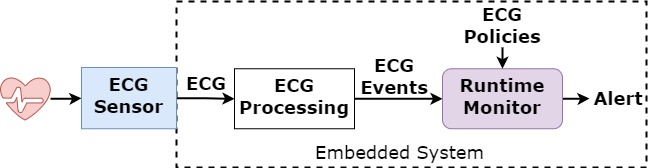
\includegraphics[width=0.5\textwidth]{Images/overview} 
	\caption{Proposed monitoring system}
	\label{monitoring_system}
\end{figure}


As seen in~\autoref{monitoring_system}, the electrical impulses of the human heart is captured by an ECG. The ECG signal is transformed into temporal events. We define policies on ECG features and specify them as timed automata (TA)~\cite{alur1994theory} which allows us to automatically synthesize an RV monitor. The monitor verifies if the incoming events satisfies the set of policies, and raises an alert if a policy is violated. Violation of policy indicates ECG/cardiac abnormality.

For the first time, we present specification, of ECG-based policies that identifies cardiac abnormalities, as TA. This enables us to synthesize formal verification monitors like RV. ECG policies and thus their TA specifications are based on Hampton's~\cite{hampton2019ecg} clinical interpretation of the primary cardiac abnormalities markers present in ECG.

%shows how the heart’s electrical impulses are recorded by an ECG. We define timed policies on ECG features to synthesize a runtime verification (RV) monitor that runs on a wearable device, classifies signals in real time, and raises an alert when abnormalities occur.

Key contributions:
\begin{itemize}
	\item We propose a formal RV monitor for classification of ECG
	enabling detection of cardiac abnormalities.
	\item We formalize ECG temporal features as a set of policies - specifying them as TA. The formally specified policies (as TA) are suitable for automated synthesis of an RV monitor.
	\item The proposed technique facilitates designing a wearable device for real-time ECG/cardiac monitoring.
	
	%\item Formalizing ECG timed features: Based on this, the set of policies based on ECG temporal features are formalized as Timed Automata (TA). The set of policies defined formally are suitable for automated analysis/synthesis of runtime monitors.
	
%	\item The proposed technique allows for designing a wearable
%	device for real-time health monitoring.
\end{itemize}